\chapter{Methodology}
This chapter details the methods used in this dissertation. Specifically, the focus is on collaborative genre tagging (CGT) - a two-step approach that applies collaborative filtering to predict genres of items such as movies or books. First, CGT is outlined and compared to more common uses of collaborative filtering on data sets such as MovieLens and Goodbooks. Then, the model architecture of CGT is detailed, along with the key hyperparameters to be tuned. Finally, the framework for hyperparameter tuning and model evaluation is described with special attention given to the reproducibility of results.

\section{Collaborative genre tagging}
Most of the previous work on collaborative filtering (CF) tackled the problem of predicting user preferences using their interaction history. The most successful methods all involve the use of latent factor models which are capable of learning otherwise hidden properties in the users and items in CF datasets. Recently this type of approach has been adapted from matrix factorisation models to neural architectures which capture latent factors in embedding layers, while allowing for non-linearity in successive hidden layers. 

CF models, by definition, do not make use of meta data for predicting user preferences -- this is the domain of content-based models. However, meta data such as item genres are still useful to users for assessing recommendations provided to them. Users cannot be expected to trust recommendations provided to them, without having some sort of description of the recommended item. While CF has shown its ability to provide recommendations to users without using content attributes, descriptive features are still useful for users to make informed decisions on \textit{which} recommendations to choose.

In this Master's dissertation, a new application of CF for predicting item genres from explicit user ratings is explored, dubbed collaborative genre tagging, or CGT. This method uses a two-headed architecture which shares a common embedding layer. The first head of the model is used to train the embedding layer, while the second head is used to learn how to predict item genres from trained embedding weights. Figure \ref{fig:4_CGT-architecture} shows the connected architecture of the CGT model.

\begin{figure}[H]
\centering
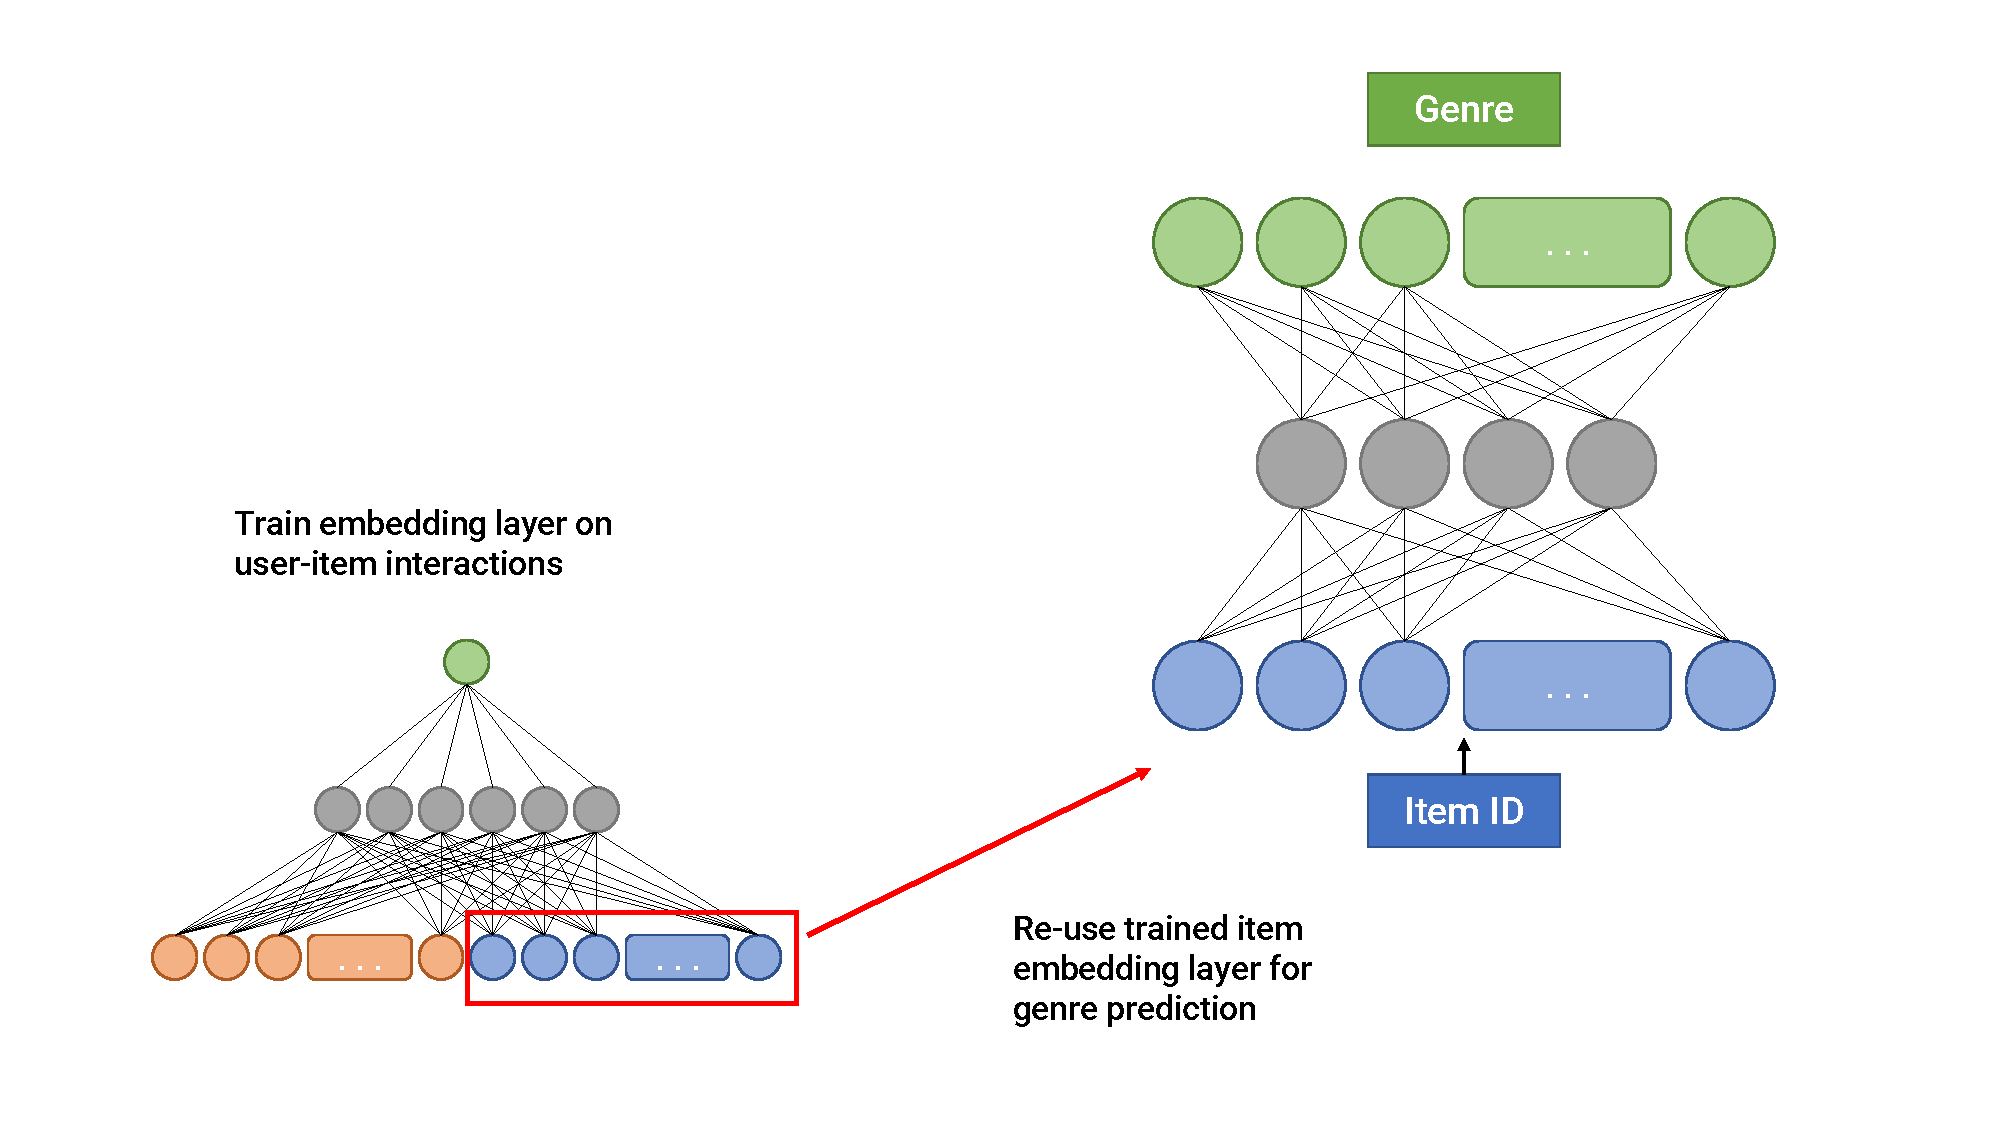
\includegraphics[width=0.95\textwidth]{Figures/4_CGT-model.pdf}
\decoRule
\caption[CGT architecture]{CGT model consists of two neural networks which share a common item embedding layer}
\label{fig:4_CGT-architecture}
\end{figure}

The first head of the CGT model uses latent factors to predict user ratings and is similar in construct to the Neural Collaborative Filtering model used by \citeauthor{he2017neural} (the architecture of which is shown in figure \ref{fig:ncf-arch}). The purpose of this model is to train the embedding layer to produce latent factors associated with every item in the ratings dataset.

After training the first head of the CGT model, the trained item embedding layer is then frozen and used as the first layer of the second head. The second head then learns a mapping from item embedding to item genre.

\section{Rating model}
\label{section:rating-model}
The rating model is the base of the CGT model. The input to this model is a user-item ID pair, and the output is an explicit rating. The IDs in the input pair are connected to an embedding layer of $k\times2$ length, where $k$ is the number of latent factors for both users and items. The embedding layer then feeds to a fully connected layer and then finally into a single output node which contains the predicted rating.

\begin{figure}[H]
\centering
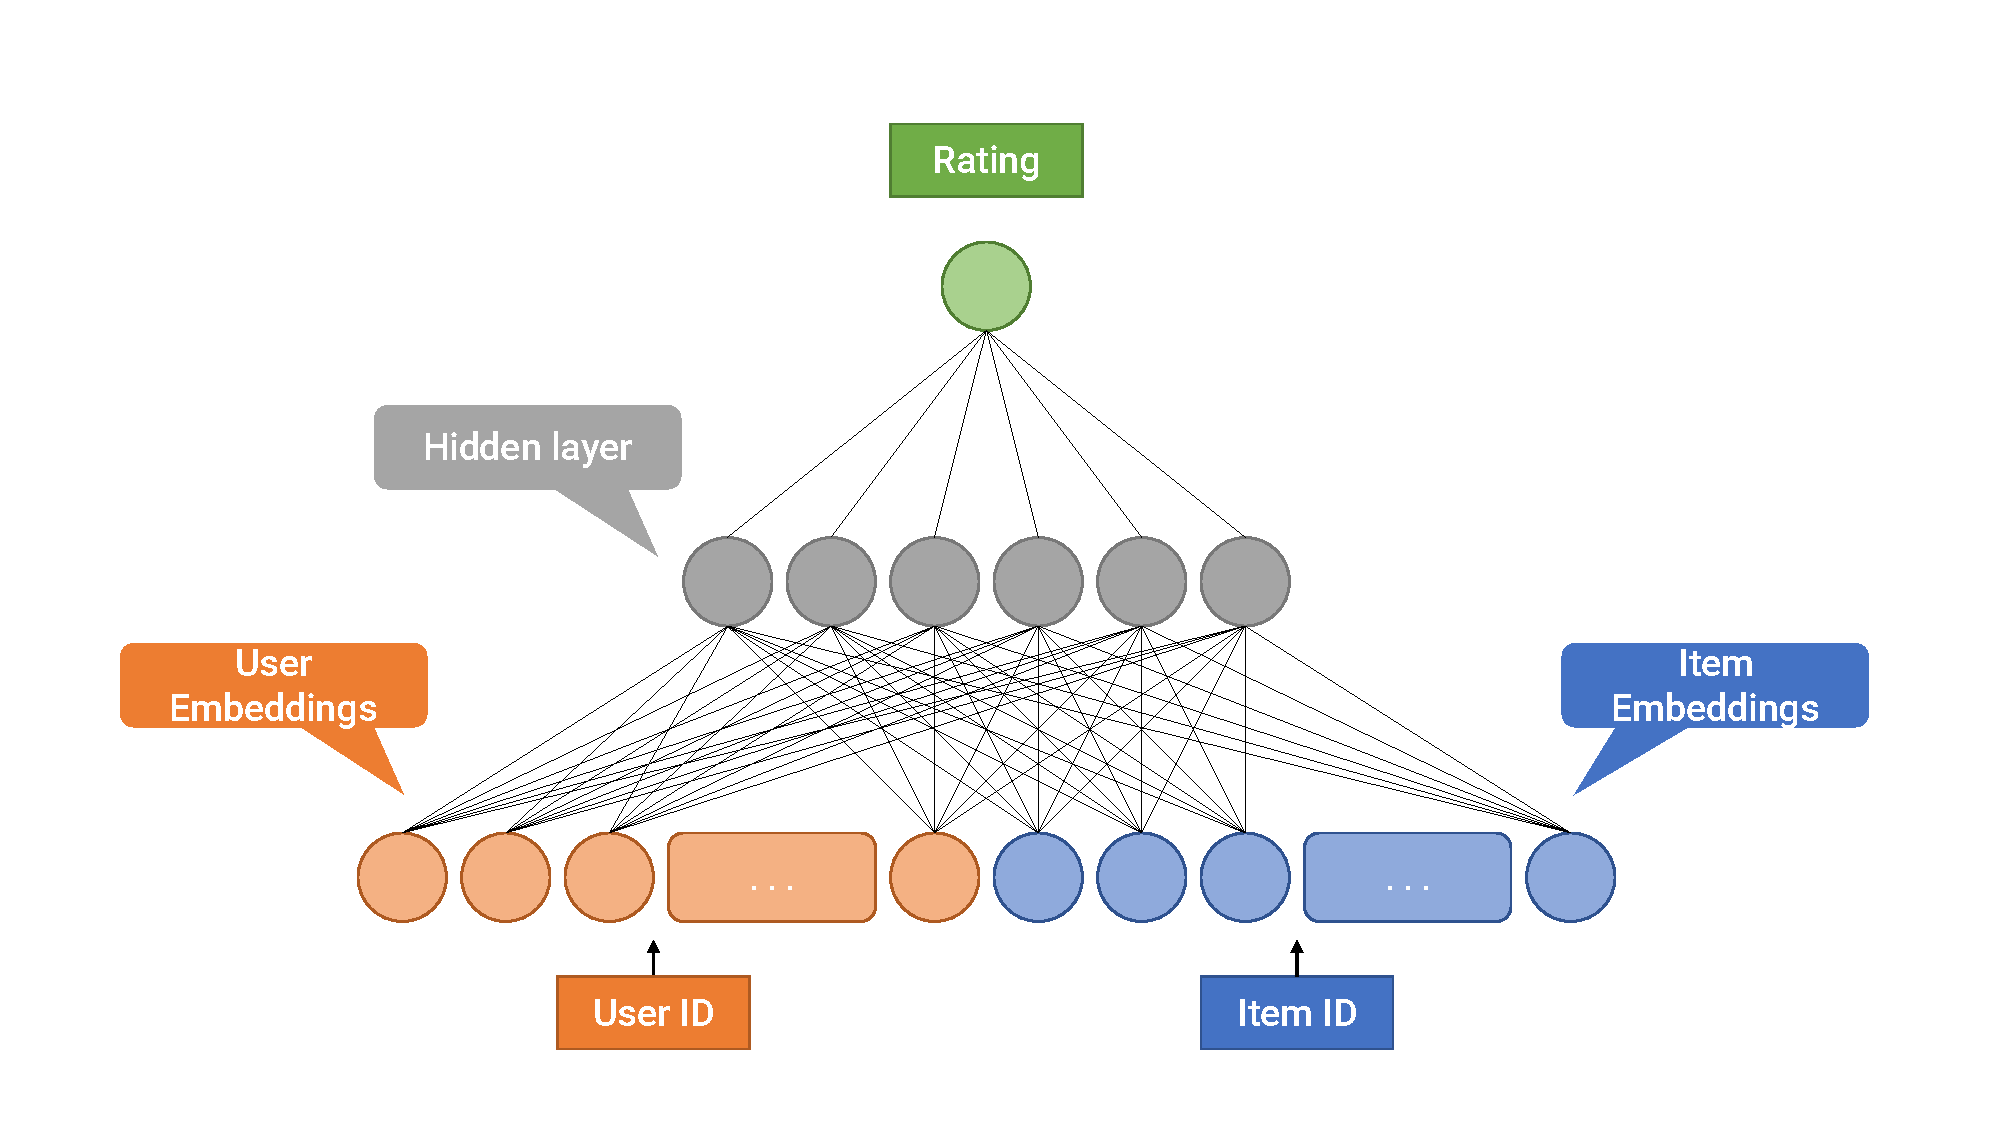
\includegraphics[width=0.85\textwidth]{Figures/4_rating-model.pdf}
\decoRule
\caption[Rating model]{Rating model uses embeddings to capture latent factors of items and users}
\label{fig:4_rating-prediction-architecture}
\end{figure}

\subsection{Embedding layer}
The first layer of the rating model is a concatenated embedding layer. This layer is comprised of two separate embedding matrices, the same as those used in the matrix factorisation method popularised by \citeauthor{koren2009matrix}. These embedding matrices hold the latent factors of all users and items respectively. The user matrix is of dimension $m\times k$ while the item matrix is $n\times k$, where $m$ and $n$ are the number of distinct users and items respectively, and $k$ is the number of latent factors.

\begin{figure}[H]
\centering
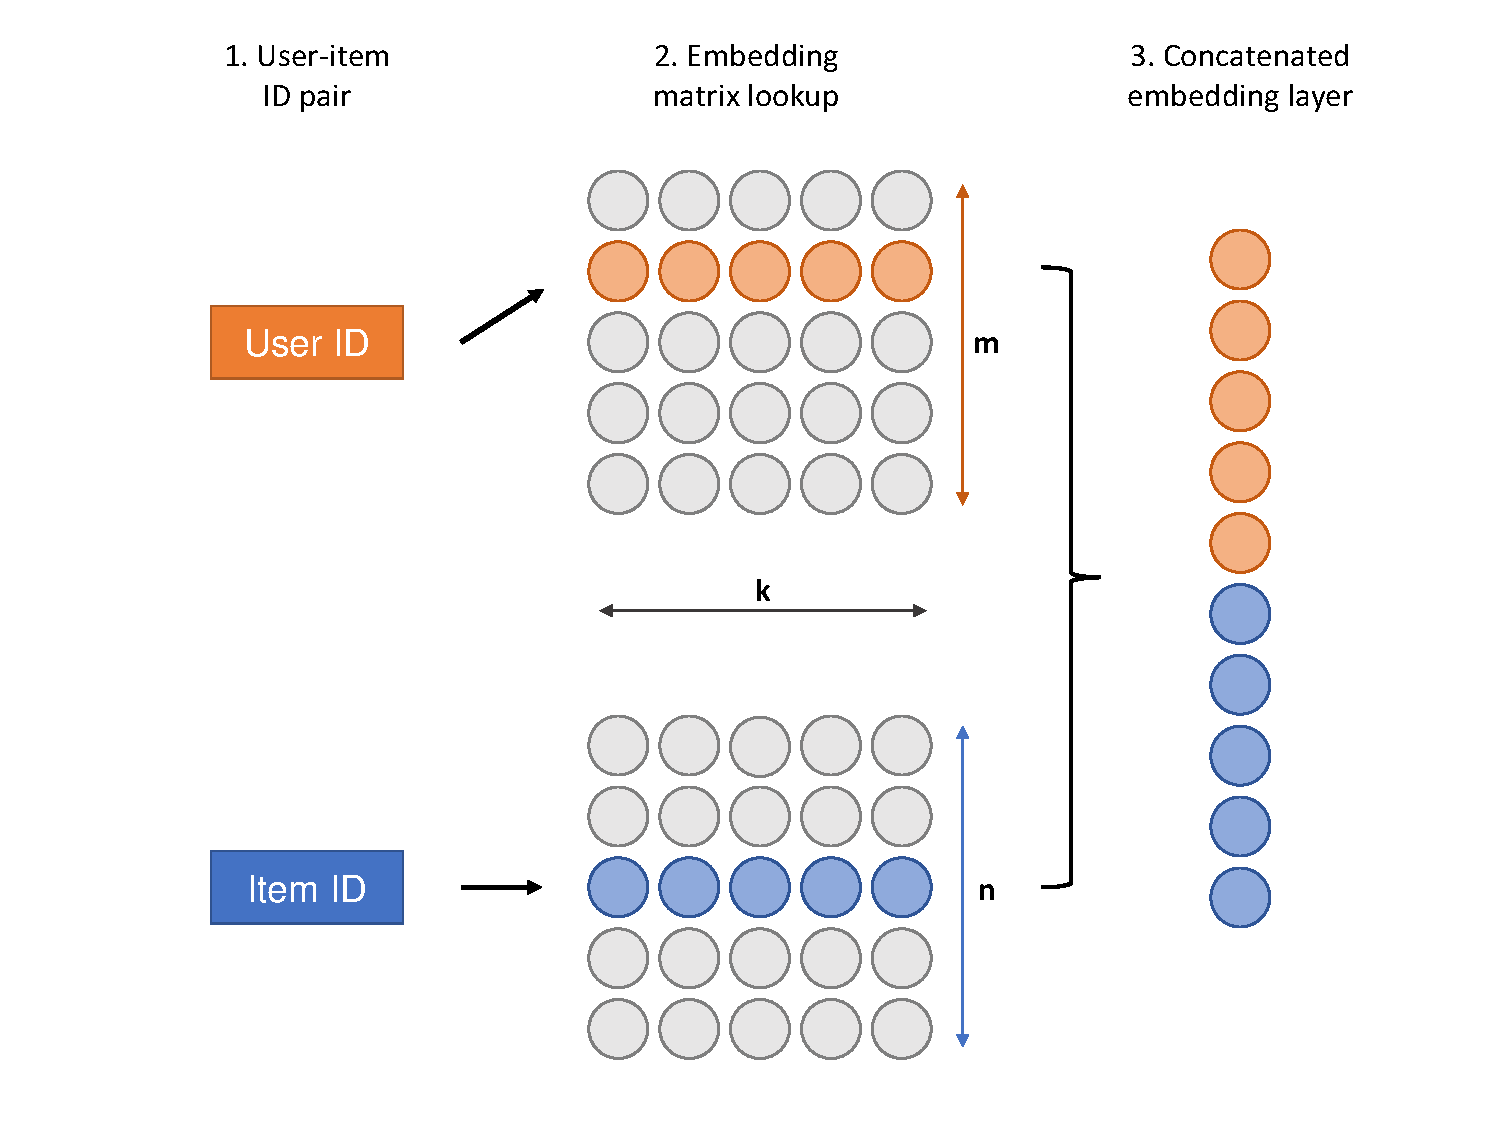
\includegraphics[width=0.8\textwidth]{Figures/4_CGT-embedding-layer.pdf}
\decoRule
\caption[Embedding layer]{Embedding layer is created as the concatenation of two separate embedding matrix lookups.}
\label{fig:4_CGT-embedding-layer}
\end{figure}

The embedding layer is the input layer of the model, which takes a user-item ID pair as its input. Each of these IDs is passed to its respective embedding matrix (step 2 in figure \ref{fig:4_CGT-embedding-layer}) as a lookup to obtain two $k$-dimensional latent factor vectors. These two latent factor vectors are then concatenated together to form the first layer of the neural network. Since each latent factor vector is of length $k$, the concatenated first layer is of dimension $k\times2$. The size of $k$ is a hyperparameter which will need to be tuned.

\subsection{Hidden layer}
The concatenated embedding layer feeds forward into the fully connected hidden layer of the model with $h$ nodes. This hidden layer allows for the model to learn non-linear patterns in the concatenated latent factor vector through the addition of activation functions. It is this non-linearity in the hidden layer that distinguishes the CGT rating model from vanilla matrix factorisation. During training of the model, dropout may also be added to this layer as a means of regularization. The number of nodes in this layer, the choice of activation function and the dropout rate are all hyperparameters that will need to be tuned.

\begin{figure}[H]
\centering
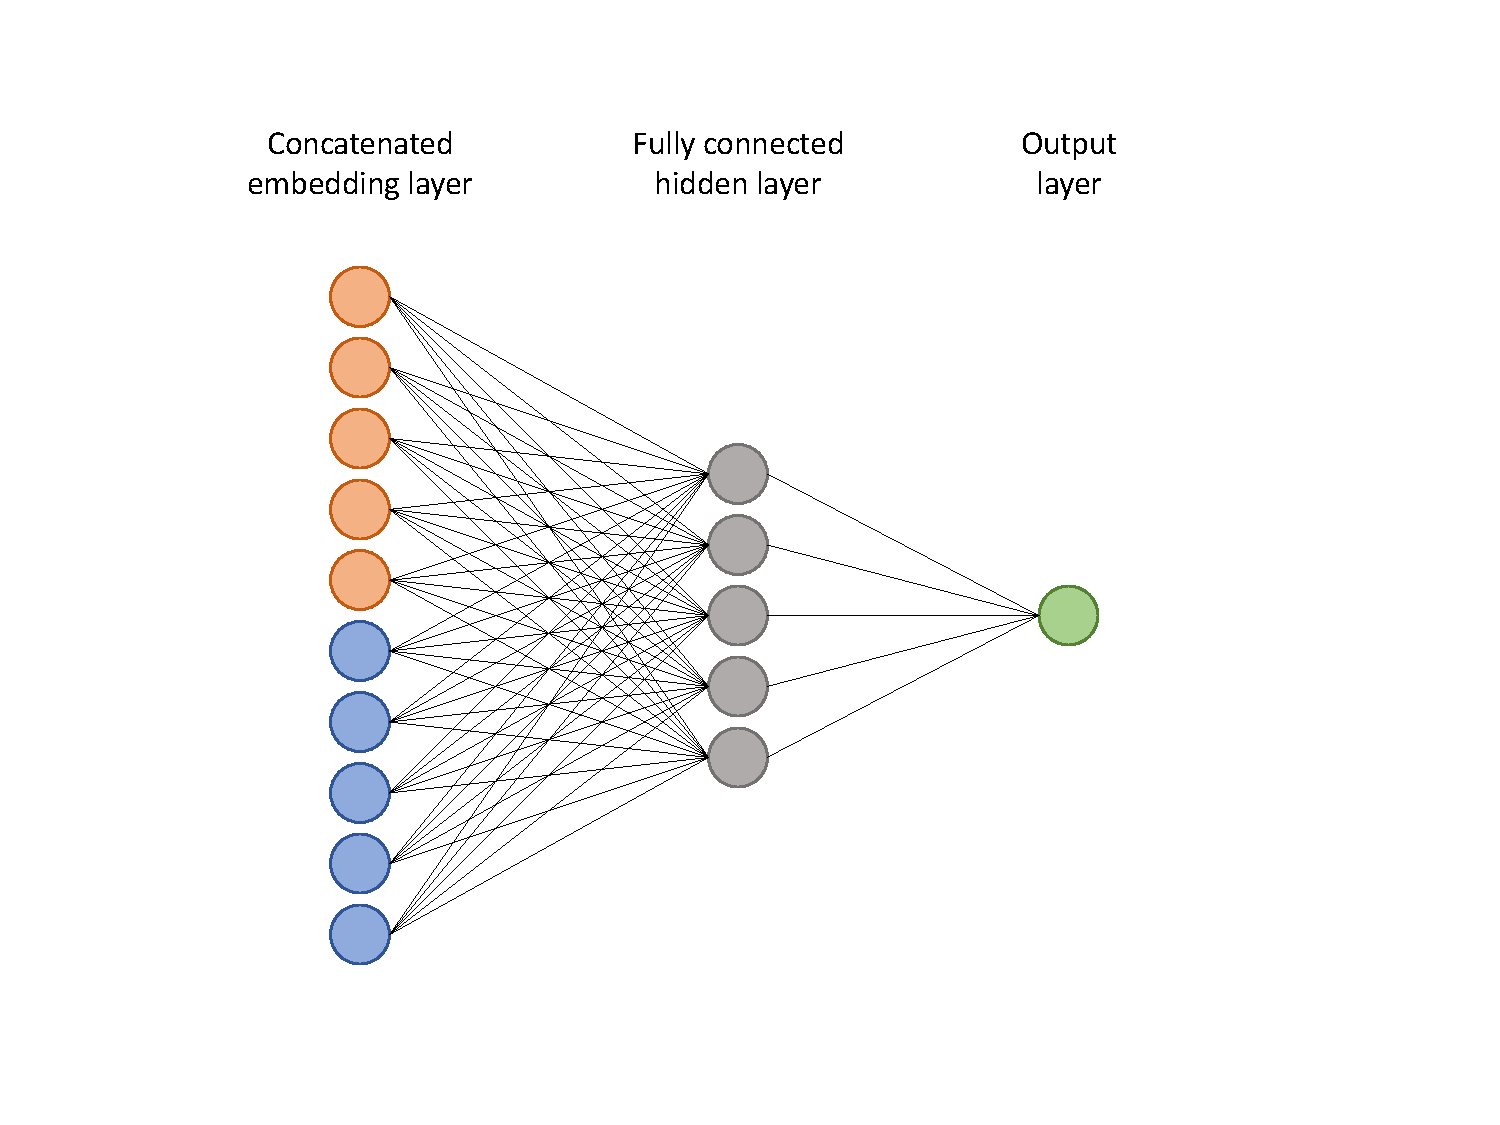
\includegraphics[width=0.8\textwidth]{Figures/4_CGT-hidden.pdf}
\decoRule
\caption[Rating model hidden layer]{Hidden layer is fully connected to concatenated embedding layer and feeds into the output node.}
\label{fig:4_CGT-hidden-layer}
\end{figure}

\subsection{Output layer}
Figure \ref{fig:4_CGT-hidden-layer} shows the full architecture of the rating model. As discussed in section \ref{section:rating-model}, the model takes two inputs: a user and an item ID. The output of the model is a predicted rating of what the input user is expected to rate the input movie. 

The network as it is shown in figure \ref{fig:4_CGT-hidden-layer} does not include any adjustments for user or item biases of any kind. \citeauthor{koren2009matrix} stated that \textit{"much of the observed variation in rating values is due to effects associated with either users or items, known as biases or intercepts, independent of any interactions."} To handle biases inherent in rating data, they adjusted their matrix factorisation model as described in equation \ref{eqn:dot_bias}.

A similar approach has been taken in the CGT model, which adjusts the model output through the addition of the global mean rating, $\mu$, and a specific user-item baseline prediction, $b_{ui}$. This adjustment is illustrated in figure \ref{fig:4_CGT-rating-layer}. 

To calculate the baseline prediction for any user-item combination, one needs to calculate the average biases for both the user and the item. The bias for a user, $u$, is calculated as 
\begin{equation}
    b_{u} = \dfrac{\sum_{j=1}^{n_u} (r_{uj})}{n_u} - \mu,
\label{eqn:CGT-user-bias}
\end{equation}
which is the average amount by which user $u$'s ratings differ from the global average rating across all users and items, $\mu$.

Similarly, the bias for an item, $i$, is thus
\begin{equation}
    b_{i} = \dfrac{\sum_{k=1}^{n_i} (r_{ki})}{n_i} - \mu,
\label{eqn:CGT-item-bias}
\end{equation}
which is the difference between the average rating from all users of item $i$ and $\mu$.

Then $b_{ui}$ is calculated as the average between the bias of user $u$ and item $i$, denoted as
\begin{equation}
    b_{ui} = \dfrac{b_u + b_i}{2}.
\label{eqn:CGT-baseline}
\end{equation}

\begin{figure}[H]
\centering
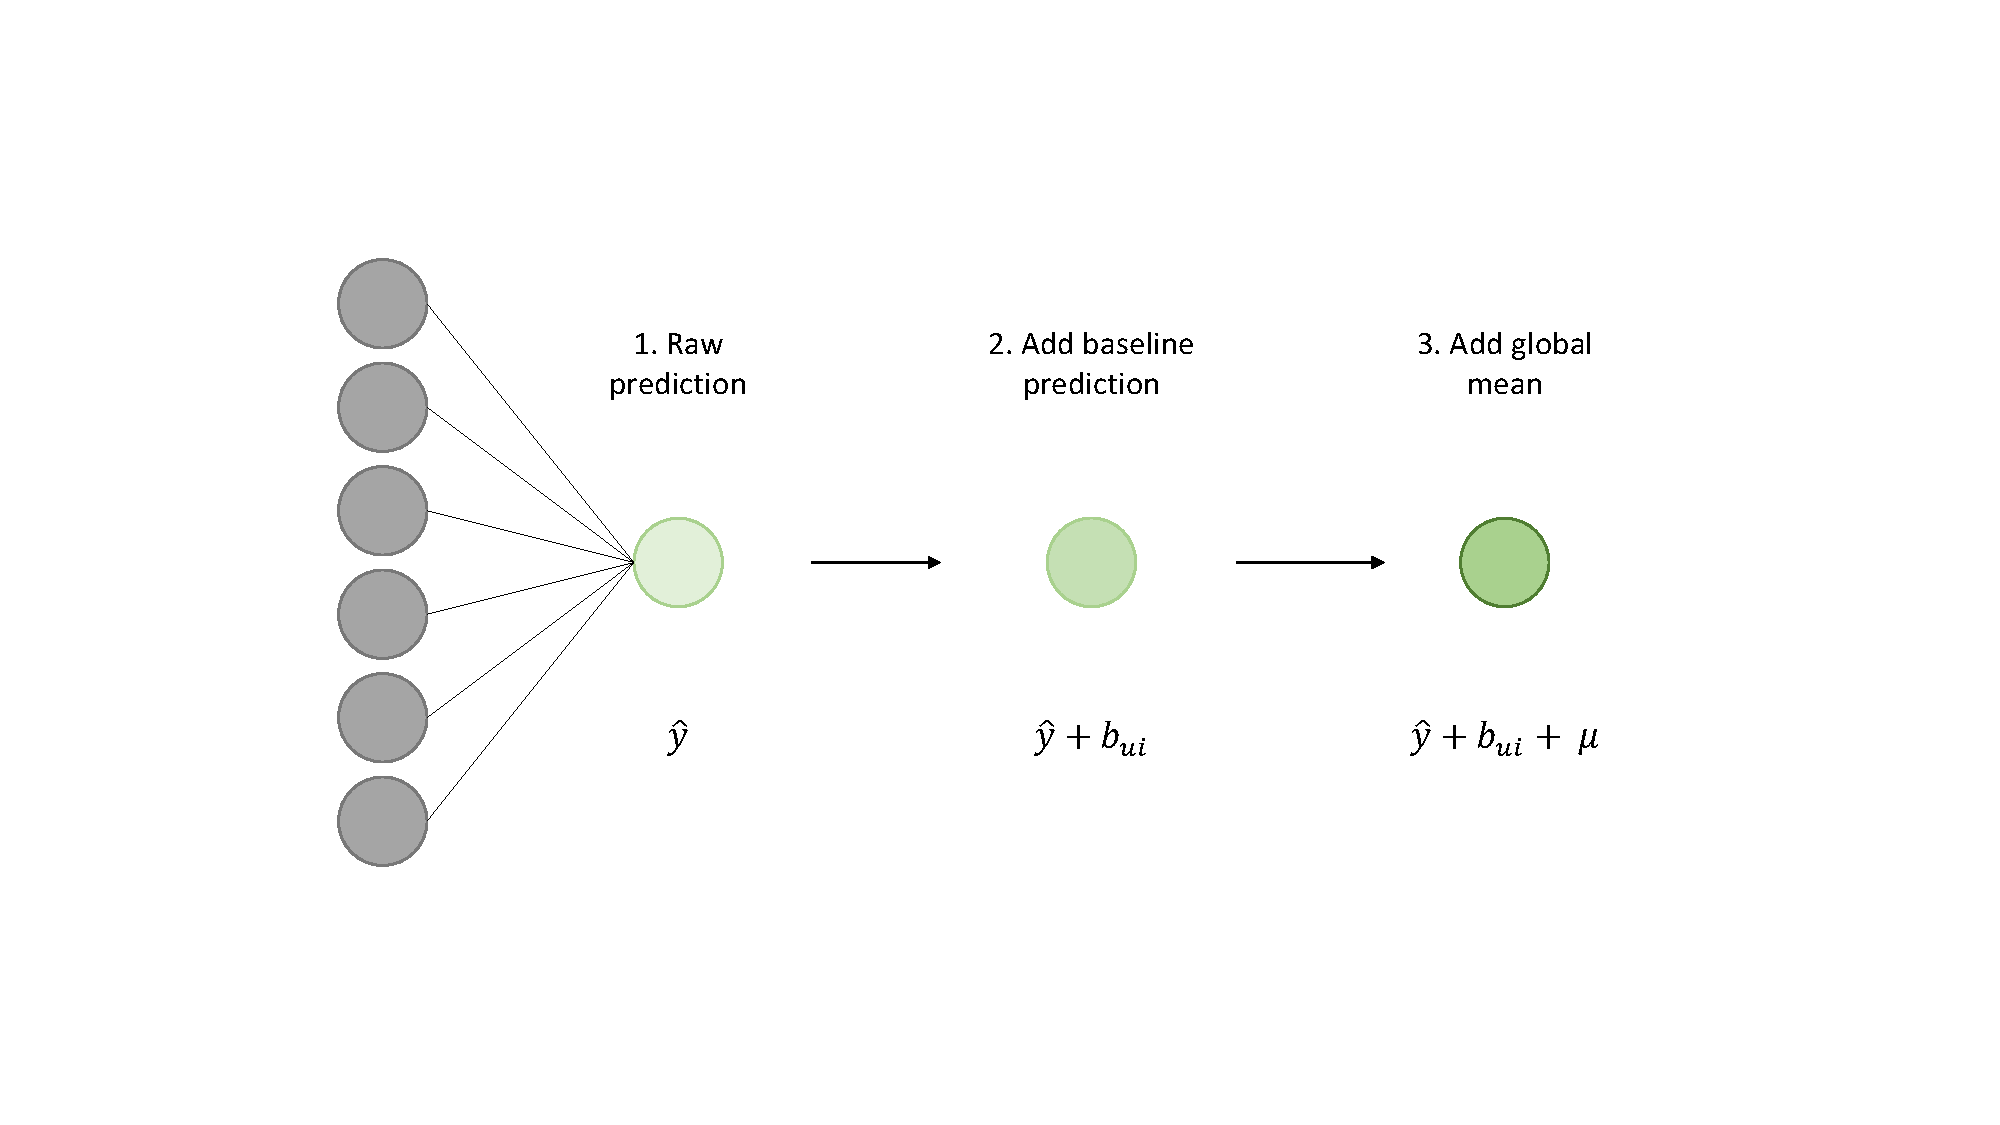
\includegraphics[width=0.9\textwidth]{Figures/4_CGT-output-layer.pdf}
\decoRule
\caption[Rating layer]{Model output is adjusted through the addition of baseline predictors.}
\label{fig:4_CGT-rating-layer}
\end{figure}

Figure \ref{fig:4_CGT-rating-layer} illustrates the addition baseline predictors to the CGT rating model. The addition of $b$ and $u$ to the output allows the model to identify the portion the rating that can be identified by biases and subjects only the "true interaction" portion of the data to the embedding and hidden layers.

The baseline predictors are not learned by the model, they are inherent in the ratings made by users of the system. The values of $b$ and $\mu$ are calculated before training the model using only the ratings from the training set. For any users or items that might appear in a holdout evaluation set but not the training set, the bias is assigned to be $\mu$.

\subsection{Summary of rating model hyperparameters}
Table \ref{tab:rating-hparams} summarises the tunable hyperparameters in the rating model. These hyperparameters were tuned and evaluated both with respect to their influence on the accuracy of the  rating model and the influence on the final genre prediction.
\begin{table}[H]
\centering
\begin{tabular}{c | p{3.5cm} | c | c}
\toprule
\textbf{Symbol} & \textbf{Description} & \textbf{Type} & \textbf{Range} \\
\midrule
$k$ & Number of latent factors in user and item latent factors & Discrete & (1, $\infty$) \\
\midrule
$h$ & Number of nodes in hidden layer & Discrete & (0, $\infty$) \\
\midrule
$dr$ & Dropout rate in hidden layer & Continuous & (0, 1) \\
\midrule
$f$ & Activation function in hidden layer & n/a & n/a \\
\bottomrule
\end{tabular}
\caption[Rating model hyperparameters]{Summary of tunable hyperparameters in CGT rating model, in the case of 0 hidden nodes.}
\label{tab:rating-hparams}
\end{table}

The standard approach to hyperparameter tuning of rating models in the past has been to use 5-fold cross validation on 90\% of the available data, with the remaining 10\% used as a true holdout set for model evaluation. The ultimate goal of CGT is to predict genres using ratings as features. The process of training the rating model can thus be thought of as a feature engineering step. It is necessary to train the CGT rating model on all available rating data, to provide items with the most descriptive latent factor vectors.

\section{Genre model}
The genre model is the second "head" of the CGT model. It re-uses the trained item embedding layer as its input layer and attempts to learn a mapping from embeddings to genres. The input layer has dimension $k$, following by a hidden layer with $j$ nodes. The output layer has as many nodes as the total number of genres with which the items have been labelled, $g$.

\begin{figure}[H]
\centering
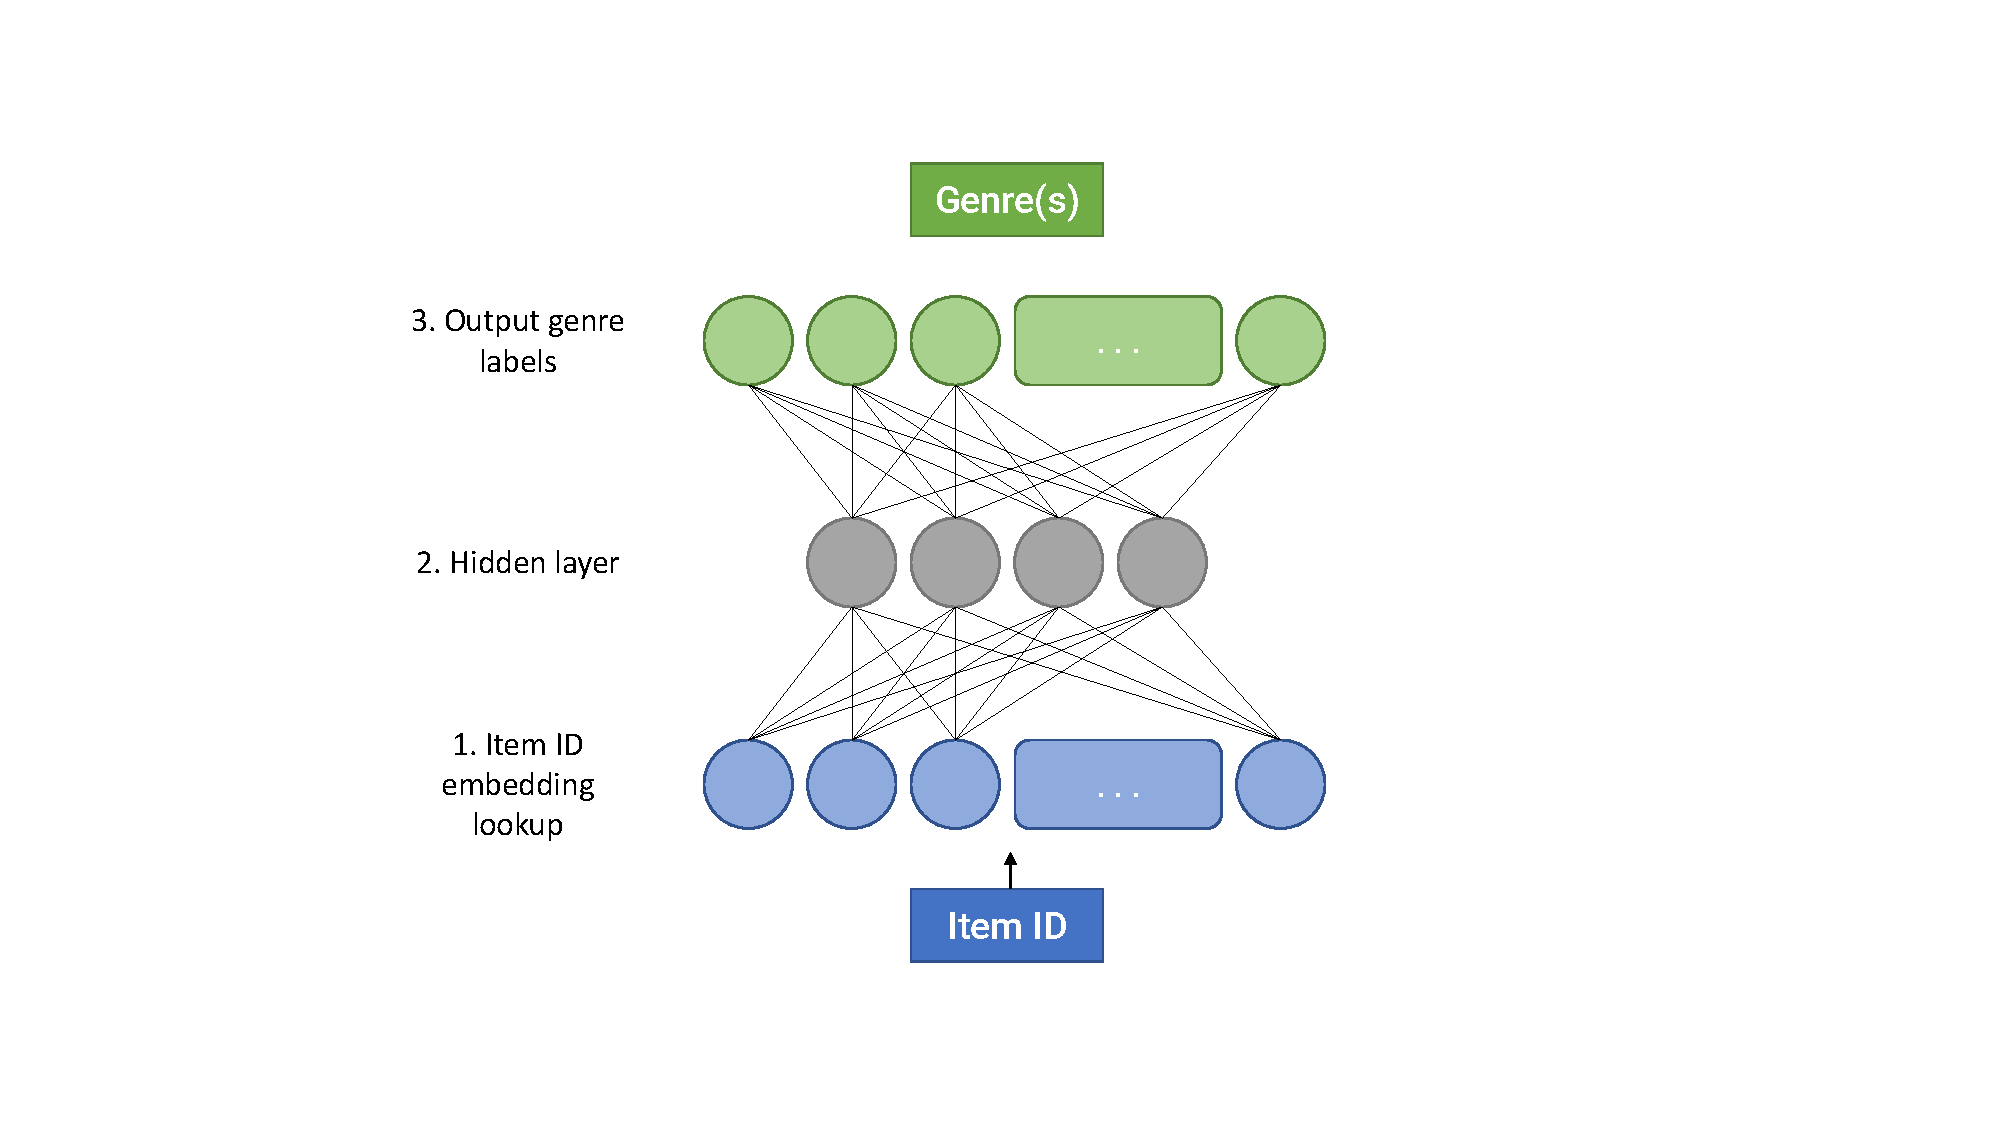
\includegraphics[width=0.8\textwidth]{Figures/4_genre-model.pdf}
\decoRule
\caption[Genre prediction model]{Genre prediction model re-uses the item embedding layer from the base ratings prediction model}
\label{fig:4_genre-prediction-architecture}
\end{figure}

\subsection{Summary of genre model hyperparameters}
\textbf{Make a table with the hyperparameters, their descriptions}